\begin{figure}[H]
    \centering
    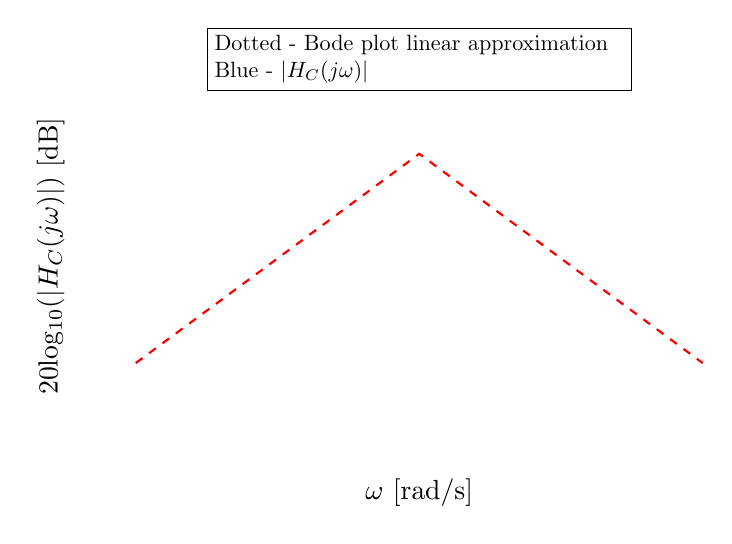
\begin{tikzpicture}[
        gnuplot def/.append style={prefix={}},
    ]
     \tikzset{
     semilog lines/.style={black},
     semilog lines 2/.style={gray!50},
     semilog half lines/.style={gray!50, dotted},
     semilog label x/.style={below,font=\small},
     semilog label y/.style={above,font=\small} }
     
    \begin{scope}[xscale=6/5,yscale=4/80]
    
    % y axis step
    \OrdBode{20}
    
    % Semilog grid
    \semilog*{3}{9}{-60}{20}
    % \BodeGraph[red!80, dashed]{3:9}{\POAmpAsymp{1}{0.000001})+\POAmpAsymp{1}{0.000001})}
    \draw [red, dashed, thick] (3,-47.16) -- (6,6) -- (9,-47.17);
    \BodeGraph{6:9} {\POAmp{2}{0.000001}}
    \BodeGraph{3:6} {-(\PIAmp{0.5}{0.000001})}
    % \BodeGraph{3:9}{-(\PIDAmp{0.5}{0.08}{0.000001})}
    
    % \BodeGraph[red!80, dashed]{-2:3}{\POAmpAsymp{100}{0.1}}
    % {20*log10(abs(sqrt(1+(0.1*10**t)**2)/sqrt(1+(100*10**t)**2)))}
    % {-\POAmp{1}{0.1}} flips over x axis center flat then down or up
    % {-\PIAmp{1}{0.1})} down or up then flat
    \node
        [rectangle, draw, fill=white, text width = 6.5cm, scale=0.8] 
        at (6,30) {Dotted - Bode plot linear approximation \\ Blue - $|H_C(j\omega)|$};
    \node[rotate=0] at (6, -80) {$\omega$ [rad/s]};
    \node[rotate=90] at (2.1, -20) {20log$_{10}(|H_C(j\omega)|)$ [dB]};
    \end{scope}
    \end{tikzpicture}
    
    \begin{tikzpicture}[
        gnuplot def/.append style={prefix={}},
    ]
     \tikzset{
     semilog lines/.style={black},
     semilog lines 2/.style={gray!50},
     semilog half lines/.style={gray!50, dotted},
     semilog label x/.style={below,font=\small},
     semilog label y/.style={above,font=\small} }
     
    \begin{scope}[xscale=6/5,yscale=4/180]
    
    % y axis step
    \OrdBode{90}
    \UniteDegre
    % Semilog grid
    \semilog*{3}{9}{-90}{90}
    % \BodeGraph[red!80, dashed]{3:9}{\POArgAsymp{1}{0.000001})}
    \BodeGraph{3:9} {90+(-(\PDArg{1}{0.000001}))-(\PDArg{1}{0.000001})}
    \draw [red, dashed, thick] (3,90) -- (5,90) -- (7,-90) -- (9,-90);
    % \BodeGraph[red!80, dashed]{-2:3}{\POAmpAsymp{100}{0.1}}
    % {20*log10(abs(sqrt(1+(0.1*10**t)**2)/sqrt(1+(100*10**t)**2)))}
    % {-\POAmp{1}{0.1}} flips over x axis center flat then down or up
    % {-\PIAmp{1}{0.1})} down or up then flat
    \node
        [rectangle, draw, fill=white, text width = 6.5cm, scale=0.8] 
        at (6,120) {Dotted - Bode plot linear approximation \\ Blue - $|H_C(j\omega)|$};
    \node[rotate=0] at (6, -120) {$\omega$ [rad/s]};
    \node[rotate=90] at (2.1, 0) {$\angle{H_{C}(j\omega)}$};
    
    \end{scope}
    \end{tikzpicture}
    \caption{Bode plot of $H_R(\omega)$}
    \end{figure}